%\section{Gesti\'on}
\begin{frame}
	\frametitle{Gesti\'on}
	
	\begin{itemize}
		\item Se han utilizado metodolog\'ias \'agiles de desarrollo
		\begin{itemize}
			\item Scrum
			\item Kanban
		\end{itemize}
	\end{itemize}
	
\end{frame}

%\subsection{Scrum}
%\begin{frame}
%	\frametitle{Gesti\'on}
%	\framesubtitle{Scrum: ¿Qu\'e es?}
%	\begin{columns}[T] % contents are top vertically aligned
%		
%		\begin{column}[T]{0.5\linewidth} % each column can also be its own 
%			\textbf{¿Qu\'e es?}
%			\begin{itemize}
%				\item M\'etodo de desarrollo iterativo e incremental
%				\item En cada ciclo de desarrollo (sprint) se genera un 
%				entregable.
%				\item Lo importante es que el diferencial de valor incremente
%			\end{itemize}
%		\end{column}
%		\begin{column}[T]{0.5\linewidth} % alternative top-align that's better 
%			%for graphics
%			\begin{figure}
%				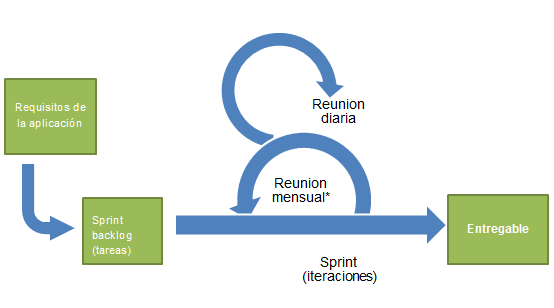
\includegraphics[width=1.0\linewidth]{./Figures/Scrumm.PNG}
%				\label{scrum}
%			\end{figure}
%			
%\tiny{\url{https://upload.wikimedia.org/wikipedia/commons/e/e5/Scrumm.PNG}
%					
%					Autor: Maxie Ayala 
%					Licenciado bajo 
%					\hyperlink{creativecommons.org/licenses/by-sa/3.0/}{CC 
%					BY-SA 3.0}}
%		\end{column}
%	\end{columns}
%
%\end{frame}
%
%%\subsection{Kanban}
%\begin{frame}
%	\frametitle{Gesti\'on}
%	\framesubtitle{Kanban: ¿Qu\'e es?}
%	
%	\textbf{¿Qu\'e es?}
%	\begin{itemize}
%		\item M\'etodo de gesti\'on del trabajo que se est\'a realizando
%		\item T\'ipicamente se utiliza un tablero o corcho con 3 columnas
%		\item Por columnas, m\'inimo se suele poner:
%		\begin{enumerate}
%			\item Qu\'e est\'a pendiente por hacer
%			\item Qu\'e se est\'a haciendo actualmente
%			\item Qu\'e se ha terminado
%		\end{enumerate}
%		
%	\end{itemize}
%	
%	
%\end{frame}

\begin{frame}
	\frametitle{Gesti\'on}
	\framesubtitle{Scrum: C\'omo se ha usado}
	
	\textbf{Ha habido 7 sprints, de un mes de duraci\'on}
	\begin{enumerate}
		\item Se ha creado un listado de tareas (Scrum backlog)
		\item Se han ordenado las tareas por prioridad
		\item Por cada sprint
		\begin{enumerate}
			\item Se seleccionan m\'aximo 3 tareas por sprint (Sprint backlog)
			\item Se desarrollan las funcionalidades
			\item Se documentan
			\item Se despliega
		\end{enumerate}
	\end{enumerate}	
\end{frame}

\begin{frame}
	\frametitle{Gesti\'on}
	\framesubtitle{Kanban: C\'omo se ha usado}
	\begin{itemize}
		\item Columna ``Por hacer": Scrum backlog
		\item Columna ``En progreso": Sprint backlog
		\item Columna ``Finalizado": Tareas finalizadas organizadas por 
		sprint
	\end{itemize}
\end{frame}